\documentclass[12pt, letterpaper, titlepage, hidelinks]{article}

% Packages
\usepackage[letterpaper, margin=1in]{geometry}
\usepackage[utf8]{inputenc}
\usepackage{fancyhdr}
\usepackage{setspace}
\usepackage{amssymb}
\usepackage{amsmath}
\usepackage{multirow}
\usepackage{array}
\usepackage{graphicx}
\usepackage{tabularx}
\usepackage{booktabs}
\usepackage{hyperref}
\usepackage{scrextend}
\usepackage{verbatim}
\usepackage[english]{babel}
\usepackage{blindtext}
\usepackage{capt-of}
\usepackage{float}
\usepackage{caption}
\usepackage{apacite}
\usepackage{mathrsfs}
\usepackage{pdfpages}
\usepackage[autostyle, english = american]{csquotes}
\MakeOuterQuote{"}

\graphicspath{ {Images/} }


\newenvironment{nospaceflalign*}
{\setlength{\abovedisplayskip}{0px}\setlength{\belowdisplayskip}{0px}%
	\csname flalign*\endcsname}
{\csname endflalign*\endcsname\ignorespacesafterend}

% Title Page
\title{4DM4 Assignment 1 \\ RISC Scheduling of the Chacha20 Stream Cipher}
\author{Ashpan Raskar raskara 400185326\\
		Ahnaf Bhuiyan bhuiya3 400198359}
\date{\today}



\begin{document}

\maketitle
\tableofcontents
\newpage
\setlength{\parindent}{0pt}
\setcounter{secnumdepth}{0}
\section{Part A}
	\subsection{A1}
		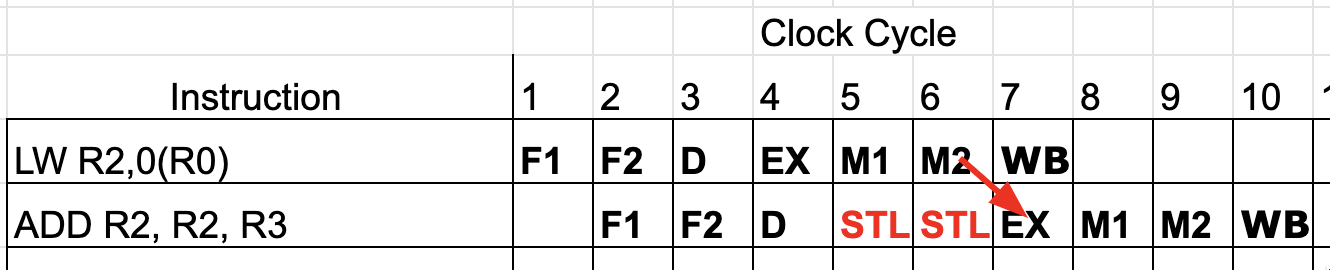
\includegraphics[width=\textwidth]{A1}
	\subsection{A2}
	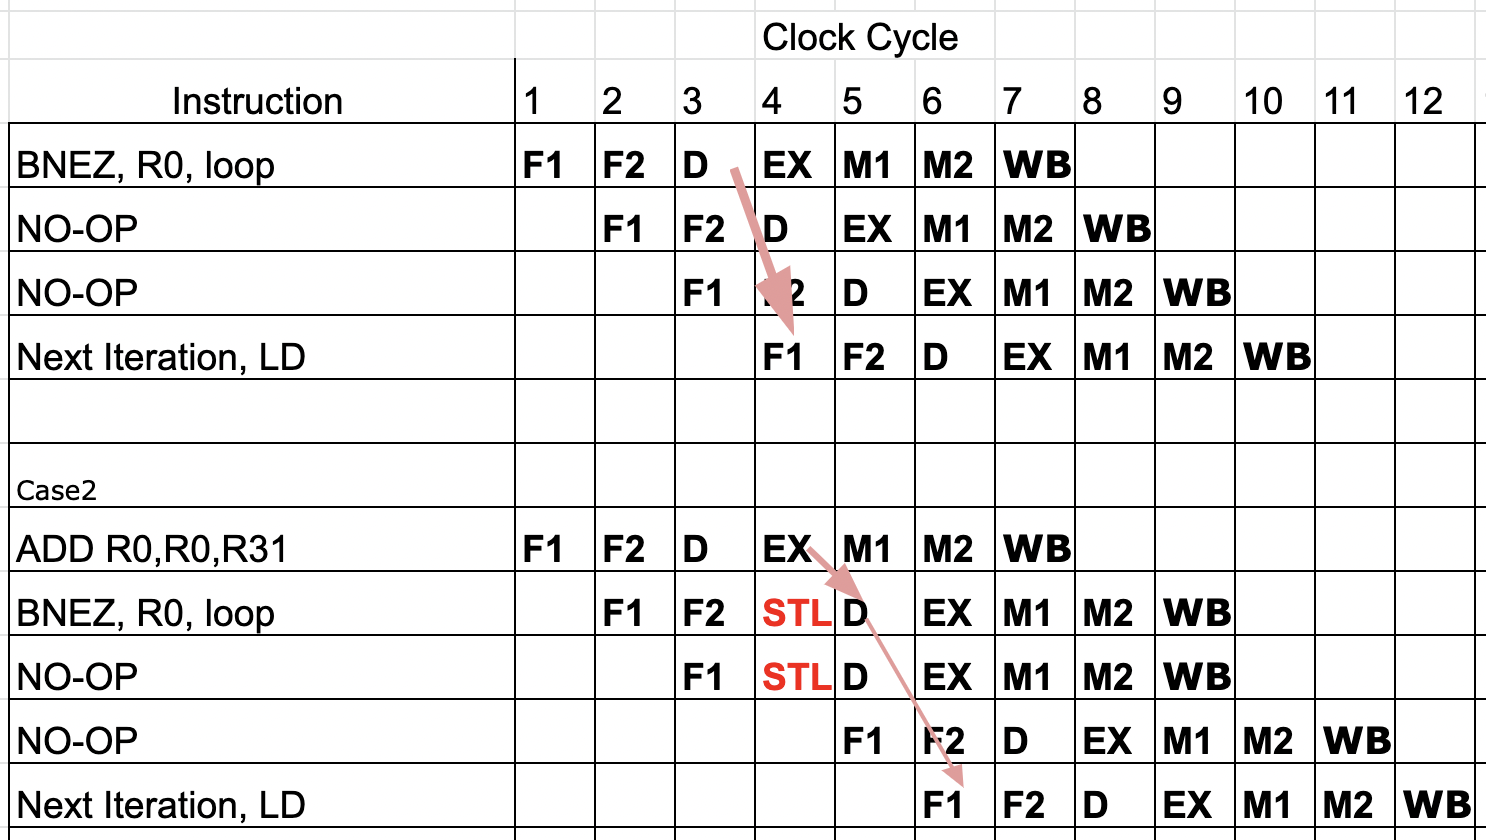
\includegraphics[width=\textwidth]{A2}
\section{Part B}
	\subsection{B1}
		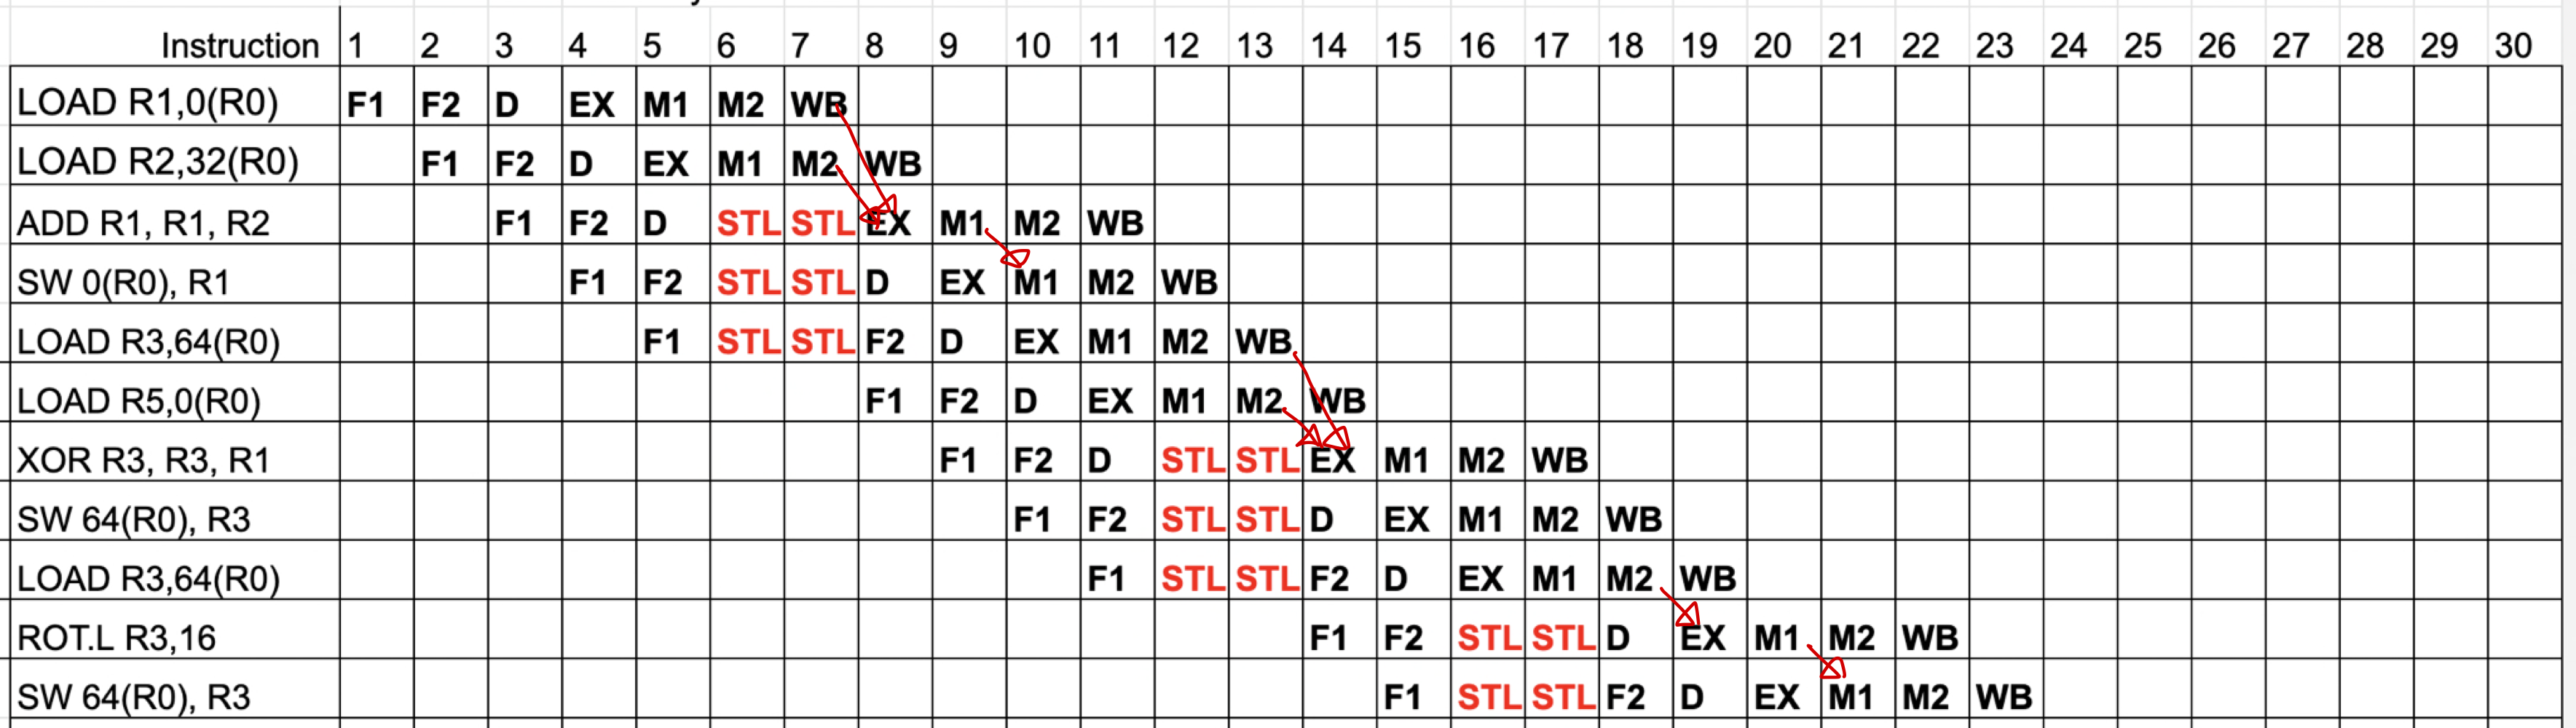
\includegraphics[width=\textwidth]{B1}
	\subsection{B2}
		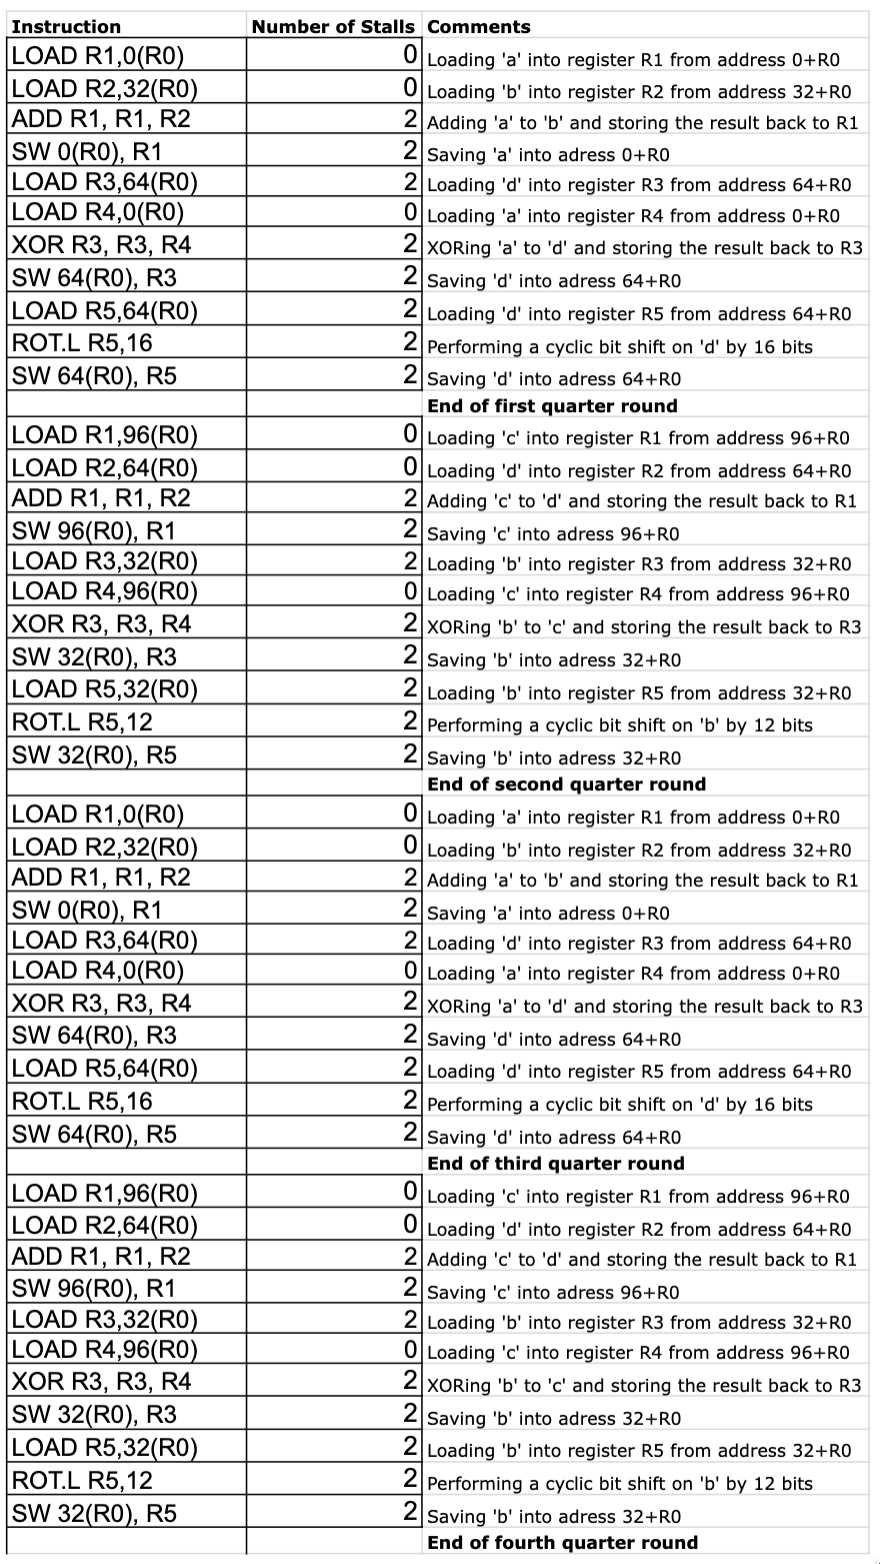
\includegraphics[width=0.8\textwidth]{B2}
	\subsection{B3}
		It takes \textbf{92 clock cycles} to complete the quarter round operation of the Chacha20 stream cipher. The number of clock cycles is calculated by adding the number of clock cycles required to complete each of the four operations in the quarter round. 
		Since one of the operations takes 23 clock cycles, the total number of clock cycles is $23 + 23 + 23 + 23 = 92$.
	\subsection{B4}
		\textbf{Assumptions}
		\begin{itemize}
			\item Assume `a' is in R2
			\item Assume `b' is in R31
			\item Assume `d' is in R30
		\end{itemize}
		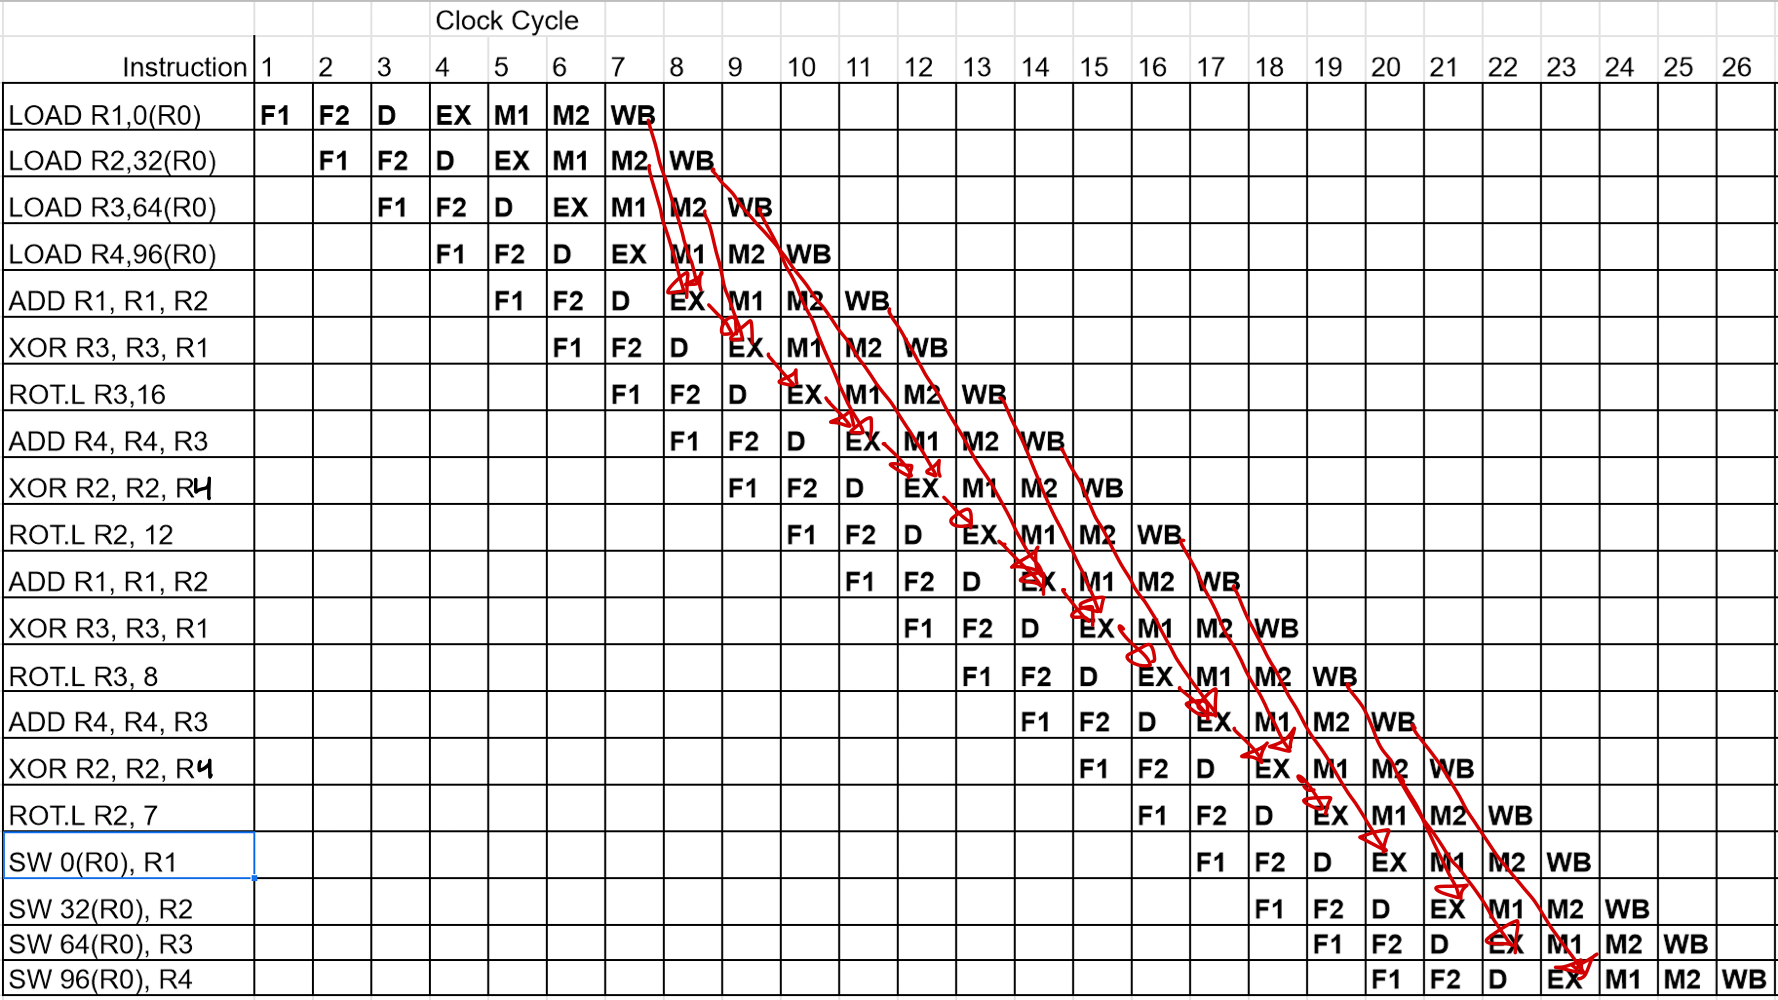
\includegraphics[width=\textwidth]{B4}
		As seen in the above table, it takes \textbf{26 clock cycles} to complete the quarter round operation. The number of clock cycles is calculated by adding the number of clock cycles required to complete each of the four operations in the quarter round, the loading and saving.
	\subsection{B5}
		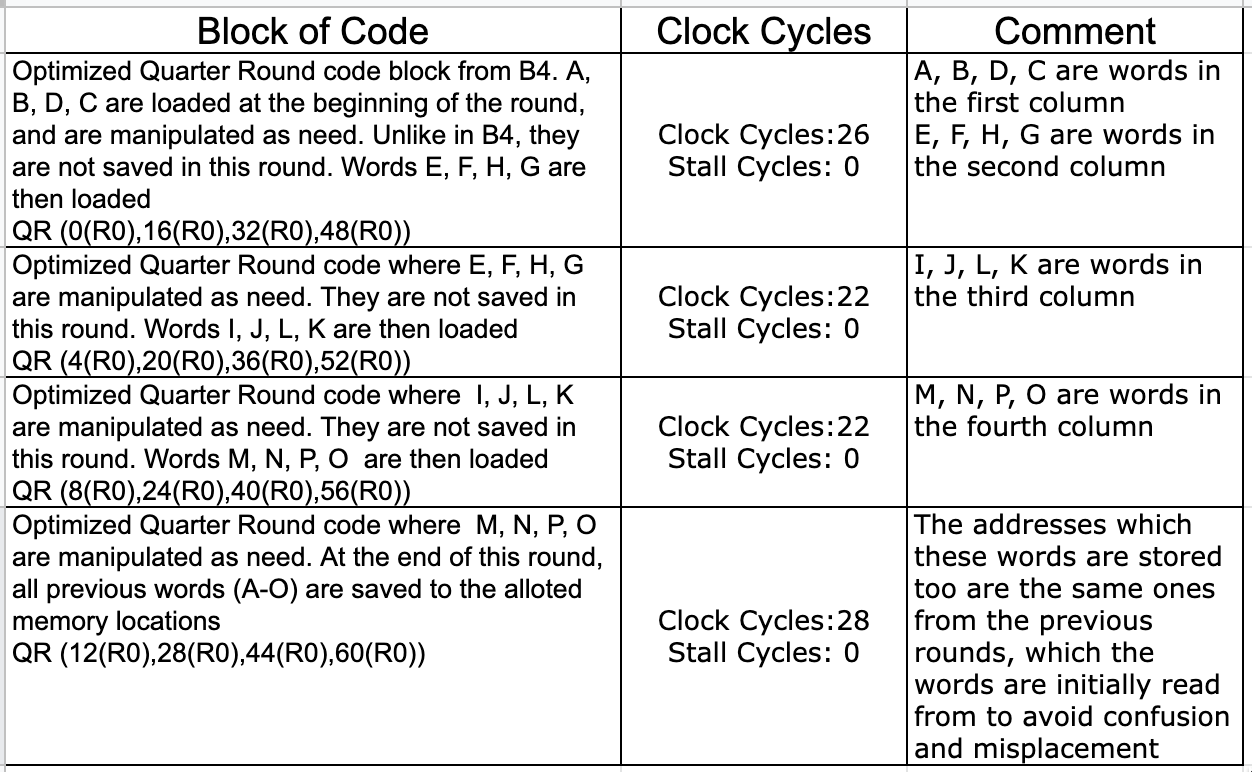
\includegraphics[width=\textwidth]{B5}
		98 clock cycles. 0 stalls.
	\subsection{B6}
		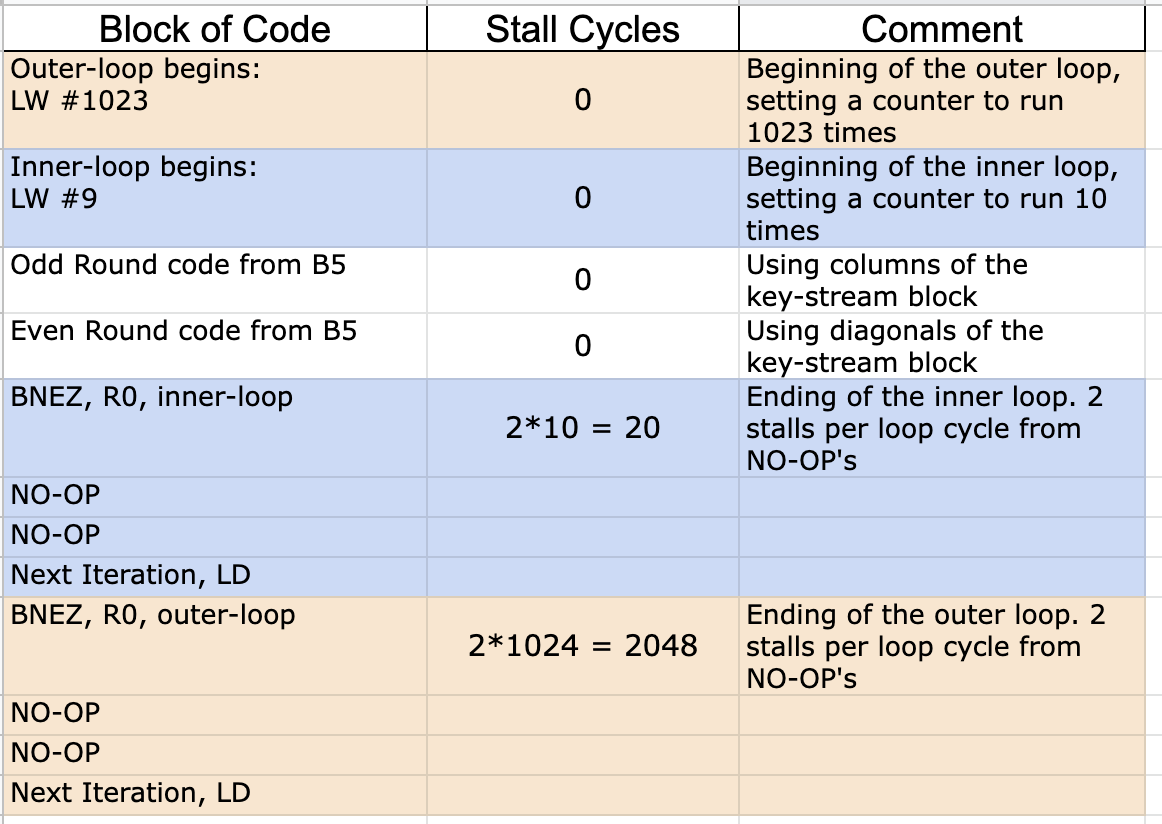
\includegraphics[width=0.8\textwidth]{B6}
		\newline
		Total clock cycles: 2131988
	\subsection{B7}
	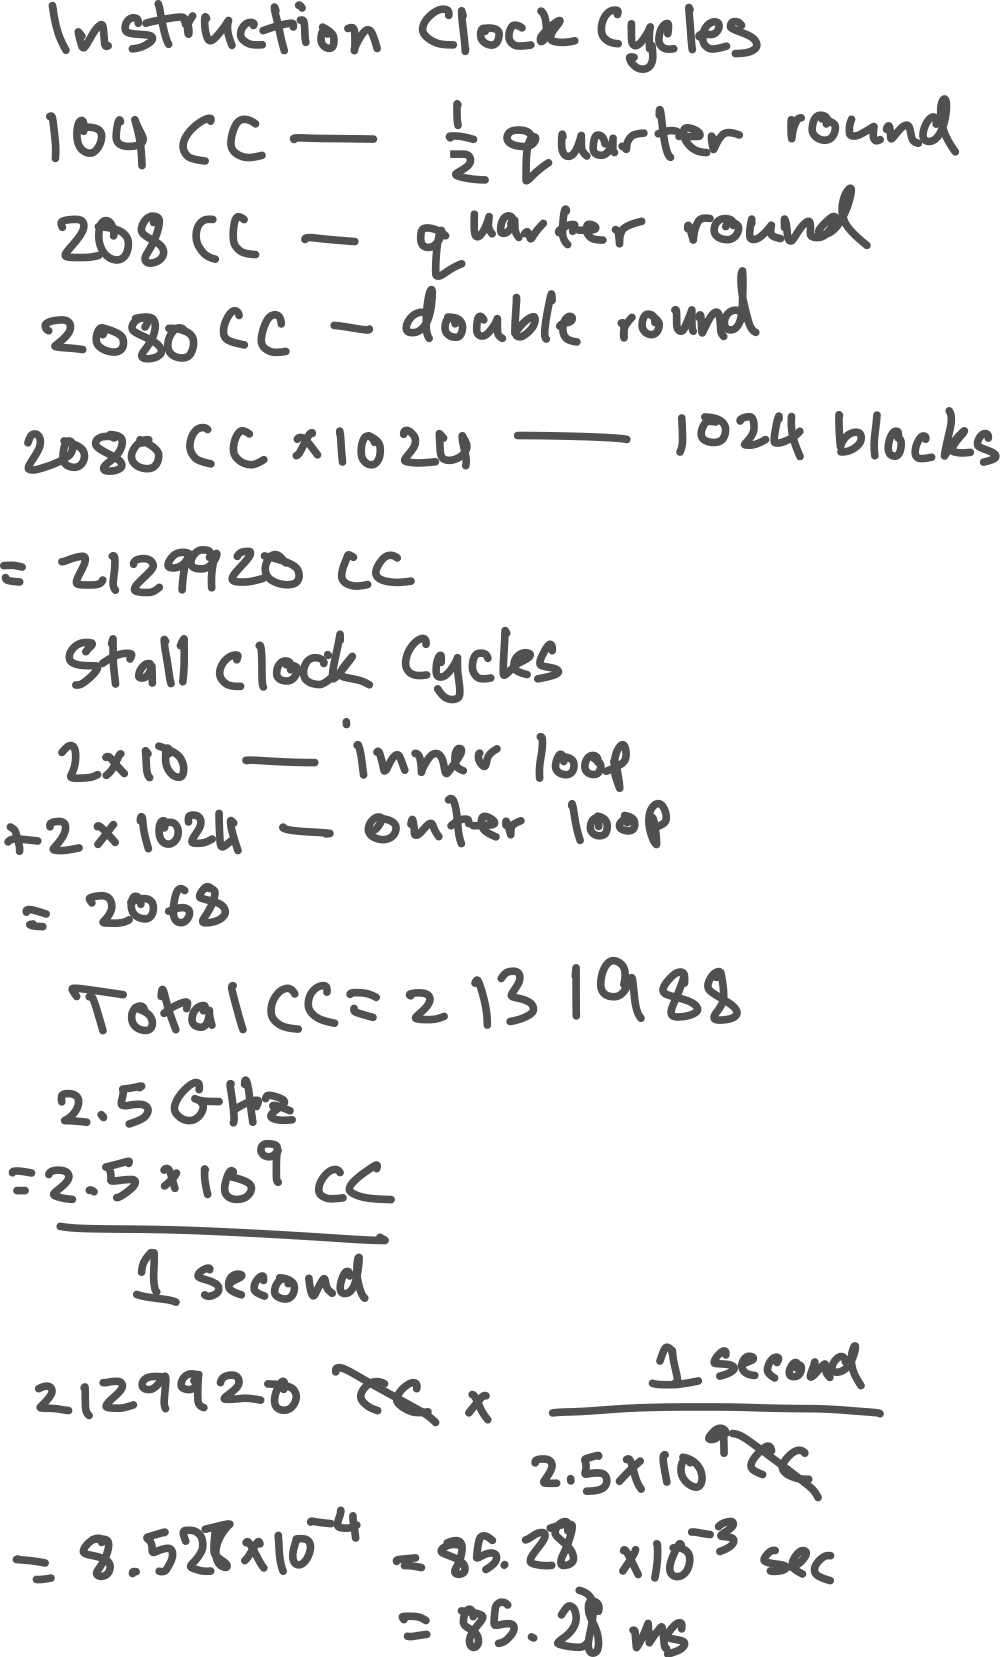
\includegraphics[width=0.7\textwidth]{B7}
	% 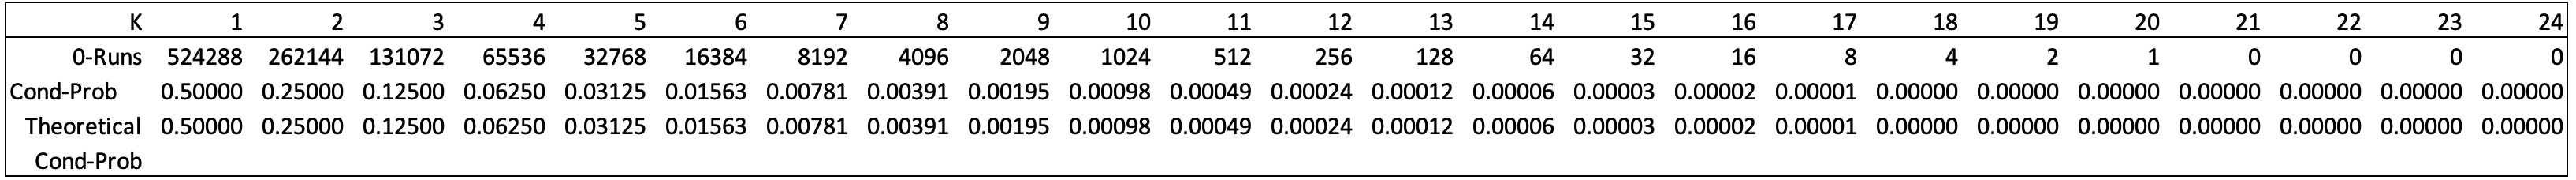
\includegraphics[width=\textwidth]{0_run_table}
\end{document}          